\begin{slikaDesno}{fig/amper_klesta.pdf}
\PID
На слици је приказан проводник у коме је успотављена стална струја јачине $I = 10\unit{A}$, обмотан са $N = 100$ навојака танког 
оптичког влакна са занемарљивим губицима. На крајевима влакна се налазе линијски поларисани фотопредајник и 
линјски поларисани фотопријемник, који су веома блиско постављени у простору. Снага светлости на 
излазу фотопредајника је $P_{\rm t} = 10\unit{mW}$. Израчунати снагу светлости коју прима фотопријемник $P_{\rm r}$. 
Вердеова константа која описује материјал од кога је израђено оптичко влакно,  
на радној таласној дужини, износи $\mathcal{V} = -160\unit{rad/(T\cdot m)}$. Осе поларизаије пријемника и предајника 
су тако постављене да важи $P_{\rm t} = P_{\rm r}$ када је $I = 0$. 
\end{slikaDesno}

\RESENJE

\noindent
\begin{minipage}[c]{0.28\textwidth}
    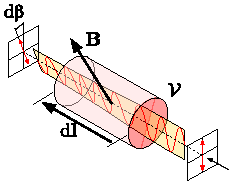
\includegraphics[scale=1]{fig/faraday.pdf}
\end{minipage}
%
\begin{minipage}[c]{0.72\textwidth}
Ротација равни поларизације приликом проласка кроз оптичко влакно узрокована аксијалним магнетским пољем 
описана је Фарадејевим ефектом. Уколико уочимо један делић влакна дужине $\de{\bf l}$, на чијем месту 
постоји магнетска индукција ${\bf B}$, на дужини тог сегмента ће се десити ротација равни поларизације 
светлости која се простире кроз влакно за угао $\de \upbeta = \mathcal{V} {\bf B} \cdot \de{\bf l}$.
Укупна промена угла поларизације може се онда одредити интеграцијом по дужини целог влакна у облику 
$\upbeta = \int_{\mathclap{\text{влакно}}} \de \upbeta = \mathcal{V} \int_{\mathclap{\text{влакно}}} {\bf B} \cdot \de {\bf l}$.
\end{minipage}
Интеграција магнетског поља по целој дужини влакна своди се $N$ интеграција по затвореној контури, чиме се има 
\begin{equation}
    \upbeta = N\mathcal{V} \oint_{\mathclap{\text{завојак}}} {\bf B} \cdot \de{\bf l}.
\end{equation}
Добијени интеграл представља циркулацију вектора $B$ по затвореној контури па је према Амперовом закону 
$\oint_{\mathclap{\text{завојак}}} {\bf B} \cdot \de{\bf l} = \upmu_0 I_{{\rm kroz} C} = \upmu_0 I$, па се коначно има 
\begin{equation}
    \upbeta = \upmu_0 N \mathcal{V} I.
\end{equation}


\noindent
\begin{minipage}[t]{0.8\textwidth}
    Ротација равни поларизација утиче на снагу коју прима поларисани фотопријемник. Интензитет светлости коју 
    прима поларизатор је $E_{\rm r} = E_{\rm t} \cos(\upbeta)$, као што је илустровано на слици. Пошто је 
    снага светлости сразмерна квадрату интензитета, то је $P_{\rm p} = P_{\rm t} \cos^2\upbeta$, па један
    коначно
\end{minipage}
\begin{minipage}[t]{0.2\textwidth}
    \vspace{0pt}
    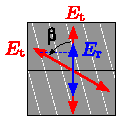
\includegraphics[scale=1]{fig/polarizacija.pdf}
\end{minipage}
\begin{equation}
    P_{\rm r} = P_{\rm t} \cos^2(\upmu_0 N \mathcal{V} I) \approx 979\unit{\upmu W}
\end{equation}